\documentclass[A4paper, 12pt]{article}
\usepackage{fancyhdr}
\usepackage{graphicx}
\usepackage{booktabs}
\usepackage{pdfpages}
\usepackage[utf8]{inputenc}
\usepackage[T1]{fontenc}
\usepackage[english]{babel}
\pagestyle{fancy}
\lhead{Vulcano 2.0: Um Novo Começo}
\rhead{v2.03 POR}
\cfoot{\thepage}
\renewcommand{\headrulewidth}{0.4pt}
\renewcommand{\footrulewidth}{0.4pt}
\addto\captionsenglish{% Replace "english" with the language you use
  \renewcommand{\contentsname}%
    {Indice}%
}
\begin{document}
\title{Vulcano 2.0: A New Beginning}
\author{The Vulcano Team}
\date{\today}
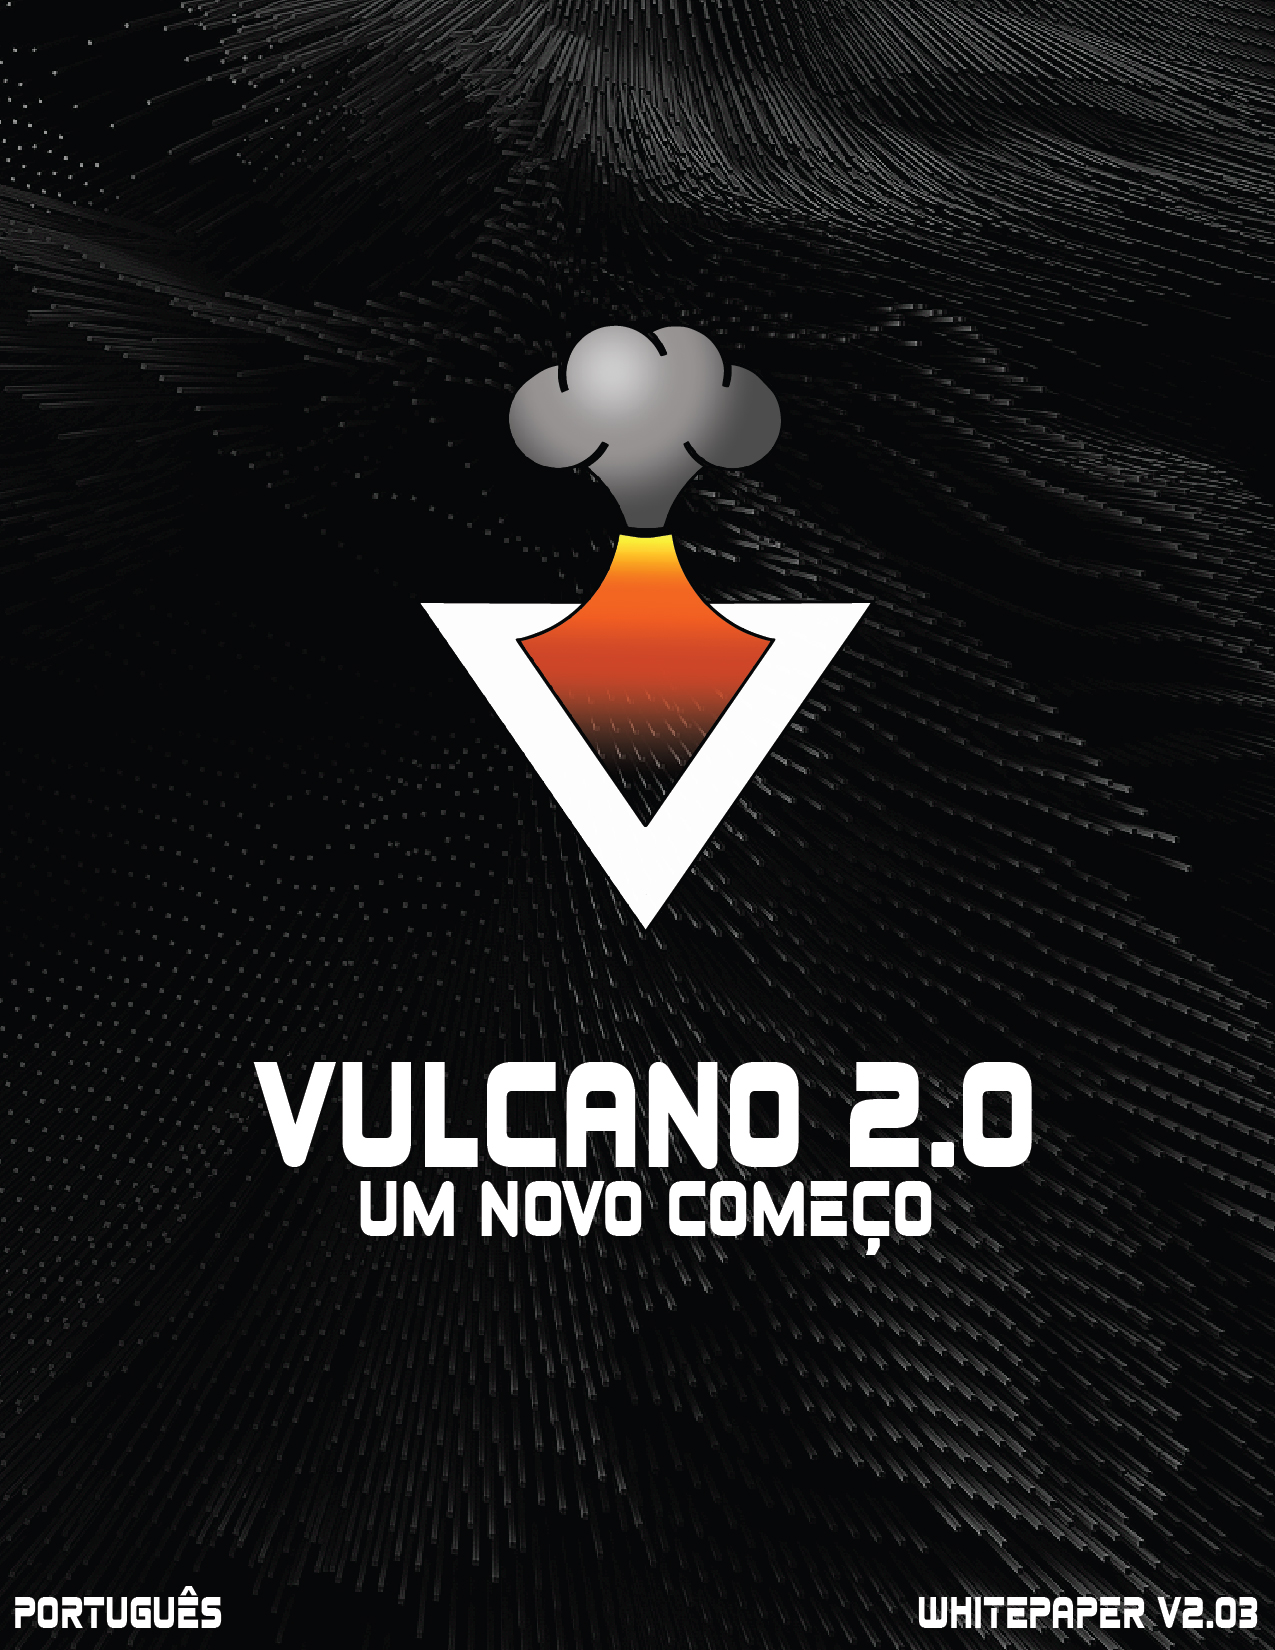
\includepdf[pages=1]{COVER-POR.jpg}
\newpage
\tableofcontents
\newpage
\section{Introdução}

Vulcano (ticker:  VULC) é uma moeda direcionada para a comunidade, criada originalmente no final de 2017 por uma equipe de desenvolvimento agora completamente retirada. Inicialmente, foi concebida apenas como uma “moeda de alto staking” com um retorno anual de 950\%.  No entanto, devido a vários erros por parte da equipe de desenvolvimento inicial, a taxa real ficou mais próxima de 320.000\%. Isso passou despercebido até que um membro da comunidade calculou essa taxa efetiva examinando o blockchain a partir do Genesis Block . Assim que esta fraqueza fundamental foi exposta, a nova equipe da Vulcano, composta por membros da comunidade, uniu-se para salvar o projeto Vulcano em um nível técnico e filosófico mediante uma reconstrução completa e o desenvolvimento de um caso de uso real. Este whitepaper estabelece uma estratégia para uma atualização total da Vulcano e um relançamento da nova moeda atualizada como meio de financiar a exploração e pesquisa geotérmica.

Em vez de simplesmente corrigir o problema da taxa percentual com a Vulcano, optamos por atualizar completamente a moeda para uma nova base de código. Para melhor modernizar o Núcleo da Vulcano, a equipe da Vulcano decidiu pela Bulwark como uma base de código. A Bulwark é construída com base na PIVX, que é construída sobre a popular criptomoeda DASH.  Esta decisão crítica nos dará a capacidade de implementar a funcionalidade masternode, governança e, eventualmente, permitir a integração de nós de hardware para suportar o ecossistema Vulcano.  Ao fazer isso, criaremos um sistema mais verdadeiramente descentralizado de governança e staking de moedas e segurança de rede.

Este artigo também delineará os planos futuros para a legitimação da Vulcano mediante da criação da Fundação Vulcano, uma planejada entidade 501(c)3 Nonprofit baseada nos Estados Unidos, que permitirá que a Vulcano cresça de forma madura e comece a se conectar e entrar em negociações com o resto do mundo dos negócios. Isso é especialmente importante, pois o caso de uso de longo prazo da Vulcano exige a aquisição de um portfólio de propriedade intelectual por meio do mecanismo de pesquisa explicado abaixo. Pela criação de um portfólio de propriedade intelectual usando o financiamento de pesquisas em universidades e instituições de pesquisa em todo o mundo. A Fundação Vulcano nos permitiria alavancar melhor essa propriedade intelectual. Este é um passo absolutamente fundamental que permitirá que o projeto Vulcano descentralizado interaja e se conecte com os mundos centralizados de empresas e academia.

Este documento também apresentará as porcentagens planejadas de taxas de governança que irão diretamente para o financiamento de pesquisa geotérmica, a fim de tanto de avançar a ciência quanto obter propriedade intelectual para trazer mais financiamento para a Fundação Vulcano para futuros desenvolvimentos e para prover verbas para subvenções adicionais.

O que você não encontrará neste documento são promessas extravagantes e sem fundamento sobre o futuro do blockchain da Vulcano.  A Vulcano busca inovação e crescimento sem fazer promessas que não possam ser cumpridas em detrimento de dedicar nossos esforços à pesquisa e ao avanço do desenvolvimento tecnológico.  Todas as tecnologias de blockchain mencionadas neste documento já foram demonstradas e serão ativadas no devido tempo.  Acreditamos que é hora de as comunidades de criptomoedas começarem a agir de maneira consistente com o potencial de negócios que exibem, e que alegações extravagantes sobre a tecnologia blockchain não são necessárias para construir um caso de negócios para o uso da tecnologia existente. Desenvolvedores, líderes de equipe e as próprias comunidades devem entender que, para sermos aceitos pelas comunidades acadêmicas e de negócios mais amplas, devemos estar dispostos a seguir suas regras até certo ponto e fazer uso efetivo do que temos antes de promover ideias sobre a tecnologia de blockchain não comprovadas, antes que tenham sido desenvolvidas, testadas e planejadas. Embora possa haver avanços na tecnologia de blockchain para a Vulcano no futuro, seu lançamento não virá com meses de fanfarra e marketing, mas só será divulgado quando já tiver sido desenvolvida. Acreditamos que este método de desenvolvimento “submarino” é o melhor para a moeda porque limita o investimento especulativo e permite a construção de uma base estável para a plataforma no futuro.

Nosso objetivo é transformar a Vulcano em uma das principais fontes de financiamento para a pesquisa de sustentabilidade no futuro e, eventualmente, construir um ecossistema de negócios em torno desta tecnologia.

\section{Agradecimentos}
A Vulcano não teria sido possível sem os trabalhos anteriores das respectivas equipes Bitcoin, Peercoin, Blackcoin, Talkcoin, Dash, PIVX e, sobretudo, Bulwark. Como a nova encarnação da Vulcano é uma ramificação modificada da Bulwark, várias seções foram emprestadas diretamente de seu whitepaper para funcionalidades que incluiremos, mas que não serão modificadas da base de código existente. Nós, a Equipe Vulcano, percebemos que seria mais transparente incluir essas seções tal como estão presentes no paper da Bulwark, em vez de reescrevê-las e fingir que são um conteúdo completamente original. Embora seja importante que nós, como comunidade, desenvolvamos casos de uso e estruturas de negócios sólidos, que funcionem para o mundo mais amplo, os princípios éticos de código aberto por trás da criptomoeda devem ser protegidos e mantidos no futuro. A humanidade, como um todo, se beneficia do compartilhamento de informações e estamos orgulhosos de contribuir para este crescente corpo de conhecimento. É com esse mesmo espírito que proporcionaremos as tecnologias desenvolvidas com financiamento por meio da Fundação Vulcano para nações que contribuem para o ecossistema de Vulcano.

\section{Uma breve introdução às criptomoedas}
Embora as propostas para a tecnologia de contabilidade distribuída remontem ao final dos anos 1980, não foi até o lançamento de um artigo, em um obscuro boletim de criptografia, intitulado “Bitcoin: Um sistema de dinheiro eletrônico ponto-a-ponto”, escrito sob o pseudônimo de Satoshi Nakamoto, que um verdadeiro blockchain nasceu. Um blockchain funciona como carimbo de data/hora sequencial para as transações e bloqueando-as em “blocos” que são validados por diversos métodos, para que não possam ser adulteradas. A Bitcoin e muitas outras criptomoedas operam com base em "Prova de Trabalho", o que significa que o poder computacional é o recurso de escassez dentro de sua rede.

No entanto, como a Vulcano está focada na sustentabilidade e na pesquisa no campo da energia, sendo um método não sustentável, é antitético para nossos esforços para aumentar a sustentabilidade. Portanto, optamos por operar com base em “prova de participação”, na qual o recurso de escassez na rede são os próprios tokens. Além disso, com o lançamento da Vulcano atualizada liberado 30 dias após a publicação deste whitepaper, também teremos os masternodes, que são uma versão um pouco mais avançada do método de prova de participação, no qual os computadores em todo o mundo mantêm a rede, mas também suportar alguma carga computacional simples para o propósito. Até o momento, essa carga computacional é pouco maior que a operação de uma carteira de staking  simples, mas gostaríamos de usar essa rede no futuro para computação distribuída para a indústria de energia renovável para a operação de problemas computacionais de química e física. Esta é um acréscimo relevante ao plano de longo prazo para a Vulcano, visto que os departamentos de geofísica e geotérmica em universidades de pesquisa, normalmente não são tão bem financiados quanto outros campos mais glamorosos e, portanto, têm maior dificuldade em obter tempo de ciclo nos grandes computadores para executar suas simulações.

Além disso, do ponto de vista do consumidor, com um tempo de bloco de 90 segundos, consenso de masternode e bloqueio de transação, um cronograma controlado e estabilizado de emissões e staking ecologicamente correto, a Vulcano aspira a ser uma criptomoeda verdadeiramente rápida e funcional, que gere um impacto real no mundo, mas também uma forte opção para os consumidores e entusiastas de criptomoedas.


\section{A Nova Vulcano}
\subsection{Especificações da blockchain Nova Vulcano}

\begin{table}[h]
\centering
\begin{tabular}{@{}ll@{}}
\toprule
Ticker & VULC \\ \midrule
Algoritmo & NIST5 \\
Porta RPC & 62541 \\
Porta P2P & 62543 \\
Espaçamento entre blocos & 90 Segundos \\
Algoritmo de Dificuldade & Dark Gravity Wave v3.0 \\
Tamanho do Bloco & 1MB \\
Maturidade minerada/cunhada & 67 Blocos ($\sim$100 Minutos) \\
Confirmation & 6 Blocks ($\sim$9 Minutes) \\
Circulação (1 Ano) & 246,194,250 \\
Circulação (5 Anos) & 421,126,225 \\
Período de PoW & nHeight: 60 \\
Período de PoS & nHeight: 61 \\
Suporte ao Protocolo & IPV4, IPV6, TOR \\
PoS & Blackcoin v3.0 PoS \\ \bottomrule
\end{tabular}
\end{table}

\subsection{Mantendo a comunidade unida}
A Vulcano foi originalmente concebida como uma moeda comunitária e esta é uma ideia em que acreditamos de todo o coração. Como uma moeda comunitária, sabemos que a melhor maneira de servir ao desenvolvimento do projeto é servir à comunidade à qual devemos nossa existência. Continuaremos nossas “chuvas”, competições e outras atividades baseadas na comunidade. Também promoveremos a discussão e a exploração dos limites do Ecossistema Vulcano. Em todos os fóruns, manteremos nossa política de tolerância zero em relação ao assédio de recém-chegados, usuários e outras comunidades de criptomoedas. A Vulcano acredita que há espaço suficiente no mundo da criptomoeda, que podemos e devemos nos esforçar para conectar e buscar sinergias, em vez de desgastar outros projetos. Embora entendamos que haja uma concorrência de boa-fé entre os adeptos das várias plataformas de criptomoeda, gostaríamos de manter todas as interações positivas.

\subsection{Desenvolvendo capacidade empresarial}
No momento da redação, houve um influxo de criptomoedas utilizando uma base tecnológica similar.  Embora a tecnologia subjacente seja sólida, muitas vezes, um exame mais profundo de suas especificações e parâmetros de blockchain revela práticas não tão justas.  Em outros casos, a implementação tecnológica é fraca, mas a comunidade não está suficientemente informada sobre os problemas para poder determinar isso e se envolver em um projeto essencialmente inconsistente.

Infelizmente, a Vulcano original poderia facilmente ter caído nessa categoria, o que é uma das principais razões pelas quais a nova equipe da Vulcano está reelaborando do zero o projeto. Acreditamos que as criptomoedas devem ter aplicações empresariais reais e que essa tecnologia não deve ser usada apenas para criar receita especulativa para um pequeno número de detentores atuando antes de o mercado entender o que realmente está acontecendo. Temos visto com frequência os desenvolvedores construírem uma moeda ruim, bombeá-la com publicidade glamorosa e depois abandonar o projeto, deixando a comunidade carregando um “mico preto”. É por isso que acreditamos na transparência e na prestação de contas e estabeleceremos a necessária base de negócios para fazer negócios reais com tanto com o mundo da criptografia quanto o da não criptografia.

Portanto, iremos estabelecer várias organizações empresariais formais para facilitar essas interações. A primeira e mais importante é a 501 (c) 3 Nonprofit que estabeleceremos com o propósito de direcionar o financiamento para iniciativas de pesquisa em geotérmica e outras ciências da terra. Esta organização será responsável pela manutenção de qualquer  propriedade intelectual e imagem de marca.

Haverá também uma série de empresas de responsabilidade limitada estabelecidas para requisitos locais em todo o mundo. Muitas permutas de criptomoeda requerem uma entidade empresarial local, e estabelecendo-se uma rede de empresas de responsabilidade limitada isso pode ser providenciado. Essa rede proporcionará à Fundação Vulcano e à comunidade Vulcano a capacidade de realizar negócios em qualquer lugar do mundo sem perder a capacidade de atender às necessidades locais e aos requisitos legais.

\subsection{Manutenção da Comunidade}
A comunidade VULC é o fator mais importante por trás do sucesso em longo prazo do projeto, e sua capacidade de influenciar significativamente o futuro da moeda e o desenvolvimento tecnológico de nossas principais áreas é primordial. Como é nosso objetivo primordial é avançar na pesquisa sobre sustentabilidade por meio do mecanismo da energia geotérmica quase ilimitada que está sob nossos pés, lançamos planos para fornecer financiamento a pesquisadores que trabalham nestas áreas.

Assim, ao final do primeiro ano, no bloco 172801, pretendemos ativar blocos de emissão de orçamento na rede.  Esses blocos de emissão, pagos mensalmente, permitirão à comunidade exercer controle significativo sobre a pesquisa que a Vulcano financia, o desenvolvimento da presença da marca e os assuntos da comunidade.  Adiar a ativação deste sistema em aproximadamente seis meses, a partir do lançamento, nos dará tempo para desenvolver a estrutura básica necessária para uma experiência positiva para o usuário e permitir que o sistema se estabilize a partir das mudanças na taxa de emissão simbólica com uma redução de 320,000\% para algo muito mais razoável.

Além disso, haverá uma estrutura de governança de 10\% adicionada a todas as retribuições de blocos que serão usadas de forma transparente e rastreável para financiar a pesquisa geotérmica. Enquanto isso continuar, utilizaremos um processo multifásico para criar e enviar propostas, além daquelas que selecionamos por nossos próprios esforços.   Para que uma proposta seja aceita, cada etapa do processo de seleção precisará ser totalmente concluída. Como acreditamos que a sabedoria e o conhecimento podem vir de uma grande variedade de locais, incentivamos a Comunidade da Vulcano a conceber as tecnologias adjacentes à Energia Geotérmica. Essas propostas e ideias serão reunidas e poderão ser votadas e discutidas pelo restante da comunidade antes de serem exploradas com maior profundidade em nível acadêmico. Esperamos que a comunidade da Vulcano possa atrair especialistas geotérmicos de todo o mundo para contribuir com esse processo de concepção.

\subsection{Taxa de emissão da Vulcano}
Abaixo estão as retribuições de bloco e taxa de emissão para o blockchain da Vulcano.
\begin{table}[h]
\centering
\begin{tabular}{@{}ccccc@{}}
\toprule
Mês & Número do bloco & Bloquear retribuição & Emitido & Total \\ \midrule
0 & 0-1 & 95,000,000 & 95,000,000 & 95,000,000 \\
1-6 & 2 to 172800 & 500 & 86,396,500 & 181,396,500 \\
7-12 & 172801 to 345600 & 375 & 64,797,750 & 246,194,250 \\
13-18 & 345601 to 518400 & 281.25 & 48,598,313 & 294,792,563 \\
19-24 & 518401 to 691200 & 210.94 & 36,448,734 & 331,241,297 \\
25-30 & 691201 to 864000 & 158.20 & 27,336,551 & 358,577,848 \\
31-36 & 864001 to 1036800 & 118.65 & 20,502,413 & 379,080,261 \\
37-42 & 1036801 to 1209600 & 88.99 & 15,376,810 & 394,457,071 \\
43-48 & 1209601 to 1382400 & 66.74 & 11,532,607 & 405,989,678 \\
49-54 & 1382401 to 1555200 & 50.06 & 8,649,456 & 414,639,133 \\
55-60 & 1555201 to 1728000 & 37.54 & 6,487,092 & 421,126,225 \\
61+ & 1728001 ao infinito & 18.77 & Continua & Continua \\ \bottomrule
\end{tabular}
\end{table}

\subsection{Trabalhando para derrotar a centralização}
Existem vários problemas endêmicos para os ecossistemas de blockchain atualmente existentes. Esses problemas, embora existam em domínios diferentes, podem ser conjuntamente descritos como excessivamente centralizados de uma maneira ou de outra.

O primeiro tipo de centralização a ser eliminado é o fato de que a grande maioria dos tokens ou moedas existentes está nas mãos de especuladores. Isso leva a oscilações completamente irracionais nos preços, à medida que vários atores tentam manipular os mercados, enquanto os especuladores desinformados que buscam a próxima "lua" compram e vendem posições rapidamente. Embora isso tenha pouco ou nenhum impacto sobre o desenvolvimento real, cria uma atitude dentro da comunidade de que as flutuações de preço de alguma forma determinam ou refletem a saúde fundamental do projeto, enquanto estão completamente desconectadas. Este problema de centralização nas mãos dos especuladores eleva à volatilidade e a um alto grau de risco. Um dos nossos objetivos é o de administrar isso tanto quanto possível.

O segundo tipo de centralização é a centralização geográfica em termos dos servidores privados virtuais sobre os quais os masternodes são tipicamente configurados. Com serviços que oferecem hospedagem masternode barata, há uma tendência para a comunidade implantar um grande número de nós em um único provedor de serviços, o que significa que um único evento imprevisto pode acabar com uma grande porcentagem da rede, conduzindo à vulnerabilidades.

Uma solução para esse problema duplicado de centralização excessiva é o Ecossistema de Pesquisas Vulcano. Como a Fundação Vulcano financia pesquisa no domínio geotérmico, espera-se que ela adquira um portfólio de propriedade intelectual. Nosso plano é o de oferecer essa propriedade intelectual a um custo muito baixo para qualquer instituição ou nação que aceite hospedar os nós de hardware da Vulcano .   Dessa forma, essas instituições terão um conjunto de ferramentas tecnológicas para usar como blocos de construção de suas próprias tecnologias pelo simples custo de implantação de masternodes em seus próprios sistemas ou em um nó de hardware Vulcano. Isso aumentará muito a distribuição geográfica dos masternodes da Vulcano, ao mesmo tempo em que também diminuirá o número de tokens flutuantes na comunidade e disponíveis para especulação.

Também consideramos que é importante que o token Vulcano esteja o mais amplamente possível distribuído. Na verdade, acreditamos que a maioria dos pequenos projetos de criptomoedas que têm grandes porcentagens de tokens nas mãos de um pequeno número de detentores introduz um grau perigoso de centralização no projeto. Portanto, pretendemos introduzir no futuro planos para incentivar a descentralização e a fragmentação de grandes carteiras e recompensar aqueles que detêm um número menor de masternodes. Isso será discutido em uma data posterior.

Como a equipe da Vulcano é uma forte defensora do desenvolvimento de código aberto, gostaríamos de manter esse modo de negócios quase de código aberto para o maior número possível de áreas. É claro que todo o código-fonte estará sempre disponível para inspeção, mas também gostaríamos de fornecer um corpo de propriedade intelectual para uso o mais barato possível.

\section{Recursos Vulcano}
\subsection {Masternodes}
Masternodes, coletivamente, são uma rede descentralizada de computadores que servem à rede Vulcano. Realizam importantes funções de rede e recebem uma parte das retribuições do bloco.  Além de atender a essas funções básicas de rede, ajudam a estabilizar o suprimento de moeda, processando transações e protegendo a rede. Masternodes exigem 50.000 VULC e conhecimentos técnicos modestos para operar. Qualquer carteira que controle 50.000 VULC pode configurar um masternode.

A equipe da Vulcano tem planos de longo prazo para a introdução de vários tipos de nós que darão retribuições com base na contribuição destes para uma rede computacional útil. Dessa forma, o desafio da “prova de trabalho” pode ser contornado quando os cálculos realizados não sejam cálculos arbitrários para proteger a rede, mas cálculos funcionais para contribuir para o avanço das ciências relacionadas à sustentabilidade. Mais informações serão divulgadas sobre essa proposta, à medida que novos desenvolvimentos ocorram.

\subsection{Ofuscação / Baralhamento de moedas}
Como o novo código Vulcano Core é baseado no Bulwark, ele também apresenta ofuscação, que é feita de forma descentralizada, facilitada pela rede de masternodes. Isso fornece uma camada adicional de privacidade nas transações. Embora não seja perfeitamente anônima, a ofuscação pelo embaralhamento de nós é muito superior à transação padrão da Bitcoin.  Por exemplo, todas as transações da Bitcoin são transparentes e podem ser facilmente seguidas através do blockchain. Para a Vulcano, um ator nocivo precisaria controlar pelo menos 50\% dos masternodes operacionais para ter uma chance superior a 0.5\% de desanonimizar uma única transação que foi embaralhada com 8 rodadas de ofuscação. Esse recurso importante fornece um alto nível de anonimato para usuários da VULC que optam por ocultar suas transações.   Embora não esteja intimamente ligado ao caso de uso final do projeto Vulcano, isso fornece um grau de usabilidade para o consumidor que aumenta seu valor em relação a outros projetos no estágio de criptomoeda.

\subsection{SwiftTX}
SwiftTX provides masternodes with locking and consensus authority for transactions. When a transaction is submitted to the network, a group of masternodes will validate the transaction. If those masternodes reach consensus on the transaction’s validity it will be locked for later introduction into the blockchain, greatly increasing transaction speed compared to conventional systems (like Bitcoin’s 10 minute block times with multiple confirmations). SwiftTX makes it possible for multiple transactions to take place before a block on the network is mined with the same inputs. This system is based on Dash’s InstantSend.

\subsection{Sporks}
A nova rede Vulcano emprega o mecanismo de bifurcação multifásica que foi introduzido no Bulwark e é conhecido como "sporking". Isso permitirá que a rede VULC implemente novos recursos, minimizando as chances de uma bifurcação involuntária na rede durante o lançamento. As alterações de spork são implantáveis via rede e podem ser ativadas e desativadas conforme necessário, sem a necessidade de atualizações de software de nó.  Esse recurso é extremamente útil e permite que a rede reaja rapidamente às vulnerabilidades de segurança, sem exigir a entrada de usuários individuais para atualizar manualmente seu código de carteira.

\subsection{TOR \& IPV6 Masternodes}
A Vulcano permitirá que o usuário execute seu nó integral ou masternode a partir de um endereço onion ou um endereço IPV6.  Estamos trabalhando para adicionar nós TOR completos para reforçar a própria rede TOR e a experiência do usuário da Bulwark, operando apenas no modo TOR. Um recurso exclusivo do suporte ao domínio TOR é poder operar seu masternode como um serviço oculto da TOR. Os nós TOR permitem que os usuários com conexões de internet estáveis operem masternodes fora de sua rede doméstica sem as implicações de privacidade de revelar sua localização ou os perigos de expor sua rede doméstica ao potencial de ataque ou comprometimento.

\section{O futuro}
\subsection{Node Hardware Seguro Vulcano}
Os principais elementos da equipe da Vulcano estão trabalhando atualmente com um fabricante especializado de eletrônicos de consumo de alta qualidade para desenvolver nós de hardware seguros que possam ser implantados globalmente para proporcionar a descentralização da rede e um maior grau de segurança. Os usuários poderão conectá-lo à sua rede doméstica e configurá-lo usando uma interface de usuário da web. As funções que pretendemos lançar com facilidade para configurar o masternode totalmente modo onion (ou nó completo), usando serviços ocultos TOR para aqueles com conexões de internet estável.

De acordo com o espírito de descentralização, todo o código-fonte estará disponível para a comunidade para montagem em casa, mas também estará disponível em um modelo pronto para uso. Esses nós também serão os nós distribuídos pela Fundação Vulcano em nosso esforço para aumentar a distribuição geográfica e o trancamento de moedas por meio da implantação de nós estáticos.

\subsection{A Loja Vulcano}
A preocupação imediata é a criação de um caso de uso do mundo real para a Vulcano. O primeiro exemplo disso será um mercado de bens digitais que opere fora do blockchain da Vulcano. Embora inicialmente seja para produtos digitais de fora da comunidade, como códigos Steam e cartões-presente, planeja-se que sejam gastos para se tornar um mercado ponto-a-ponto baseado na Vulcano.

\subsection{Telegram \& Botões de Discord}
A alma de todo projeto de blockchain é a comunidade, e uma das melhores maneiras de servir a comunidade é proporcionando uma maneira de se comunicar e usar o token. A equipe da Vulcano financiará a criação de bots para vários serviços de bate-papo que permitirão que as pessoas compartilhem seu VULC facilmente com o resto do mundo.  Pela facilitação deste fluxo livre da Vulcano, podemos melhorar a utilidade ao mesmo tempo em que também envolvemos e desenvolvemos a comunidade.

\section{Conclusão}
A Vulcano está muito longe de onde estava quando as fraquezas críticas foram descobertas há vários meses. Os testes estão sendo conduzidos na nova rede Vulcano, seus recursos estão sendo ampliados e muito trabalho já foi feito para consertar os problemas que afetaram o projeto e a comunidade por meses.  Temos o prazer de anunciar essas mudanças e atualizações e estamos contentes em revelar nossos planos de longo prazo. Este whitepaper deve ser um documento vivo e esperamos realizar atualizações contínuas.
\newpage
\section{Changelog}

\begin{table}[h]
\centering
\begin{tabular}{@{}ccccc@{}}
\toprule
Versão & Data & Explicação \\ \midrule
v2.03 & August 8th, 2018 & Primeira Tradução em Português \\
 \bottomrule
\end{tabular}
\end{table}

\end{document}
